\documentclass[11pt,a4paper]{article}
\usepackage[utf8]{inputenc}
\usepackage{amsmath,amssymb,amsthm}
\usepackage{graphicx}
\usepackage{booktabs}
\usepackage[margin=2.4cm]{geometry}
\usepackage{hyperref}

\newtheorem{prop}{Proposition}
\theoremstyle{remark}
\newtheorem*{rem}{Remark}

\newcommand{\R}{\mathbb{R}}
\newcommand{\bb}{\mathbf{b}}
\newcommand{\x}{\mathbf{x}}
\newcommand{\z}{\mathbf{z}}

\title{Playing styles and balanced training groups\\
\large PCA, the power method and variance decomposition\\ applied to a rugby squad}
\author{Matteo Guerrucci}
\date{Numerical Analysis project --- September 2026}

\begin{document}
\maketitle

\begin{abstract}
A squad of $N=25$ players is described by $D=10$ statistics per 80 minutes.
Principal component analysis (PCA) identifies a few \emph{playing-style axes};
the components are computed with a power method implemented from scratch, with deflation,
and checked against the SVD. In the style space the squad is then split into 5
\emph{balanced} training groups by minimising the between-group variance: by the variance
decomposition this is equivalent to mixing, in every group, players who are strong and weak on
every axis. Finally, each player is compared with the mean of their role to derive individual
work directions and an in-group mentor. The data are synthetic.
\end{abstract}

%=====================================================================
\section{Background: expected value, variance, covariance}
Reference: M.~P.~Deisenroth, A.~A.~Faisal, C.~S.~Ong, \emph{Mathematics for Machine Learning},
Cambridge University Press, 2020 (ch.~6, summary statistics; ch.~10, PCA). The book uses the
convention $X\in\R^{D\times N}$ (data by columns) and the factor $1/N$; here $X\in\R^{N\times D}$
(one row per player) and $1/(N-1)$, the unbiased estimator.

\paragraph{Expected value and variance.}
For a random variable $x$ with mean $\mu=\mathbb{E}[x]$:
\[
\mathbb{V}[x]=\mathbb{E}\big[(x-\mu)^2\big]=\mathbb{E}[x^2]-\big(\mathbb{E}[x]\big)^2,
\qquad \sigma=\sqrt{\mathbb{V}[x]}\ \ \text{(standard deviation)}.
\]
For a random vector $\x\in\R^D$ with mean $\boldsymbol\mu$, the covariance matrix is
\[
\Sigma=\operatorname{Cov}[\x]=\mathbb{E}\big[(\x-\boldsymbol\mu)(\x-\boldsymbol\mu)^T\big],
\qquad \Sigma_{ij}=\operatorname{Cov}[x_i,x_j],\quad \Sigma_{jj}=\mathbb{V}[x_j].
\]
\paragraph{Empirical versions.} From $N$ observations $\x_1,\dots,\x_N$:
\[
\bar\x=\frac1N\sum_n\x_n,\qquad
C=\frac{1}{N-1}\sum_n(\x_n-\bar\x)(\x_n-\bar\x)^T=\frac{1}{N-1}X^TX\ \ (X\text{ centred}).
\]

\paragraph{Why we centre first: a numerical fact.}
The two expressions of the variance are equal in exact arithmetic, but not in floating point.
$\mathbb{E}[x^2]-(\mathbb{E}[x])^2$ subtracts two large, nearly equal numbers: this is
\textbf{catastrophic cancellation}. With the values $\{4,7,13,16\}$ (exact variance $22.5$) shifted
by $10^9$, the one-pass formula gives $-128$ (a negative variance), the two-pass formula
$\mathbb{E}[(x-\mu)^2]$ gives $22.5$. This is why the code always centres the data before computing $C$.

\paragraph{Linear transformations.}
If $\mathbf y=A\x+\mathbf c$, then
\[
\mathbb{E}[\mathbf y]=A\boldsymbol\mu+\mathbf c,\qquad \operatorname{Cov}[\mathbf y]=A\,\Sigma\,A^T .
\]
In particular, for the projection onto a direction $\bb$ ($A=\bb^T$):
\[
\boxed{\ \mathbb{V}[\bb^T\x]=\bb^T\Sigma\,\bb\ }
\]
is the starting point of PCA: the variance along a direction is a quadratic form in the
covariance matrix. With $B^T$ in place of $\bb^T$: $\operatorname{Cov}[B^T\x]=B^T\Sigma B$.

\paragraph{Geometry of random variables.}
For zero-mean variables, $\langle x,y\rangle:=\operatorname{Cov}[x,y]$ is an inner product.
The induced norm is the standard deviation, $\|x\|=\sqrt{\operatorname{Cov}[x,x]}=\sigma_x$, and
\[
\cos\theta=\frac{\langle x,y\rangle}{\|x\|\,\|y\|}=\frac{\operatorname{Cov}[x,y]}{\sigma_x\sigma_y}=\rho(x,y),
\]
that is, \textbf{the correlation is the cosine of the angle} between the two variables.
\textbf{Uncorrelated} variables are \textbf{orthogonal}. In this geometry PCA looks for orthogonal
directions: the scores along different components are uncorrelated, because
$\operatorname{Cov}[\bb_i^T\x,\bb_j^T\x]=\bb_i^T\Sigma\bb_j=\lambda_j\bb_i^T\bb_j=0$ for $i\ne j$.
Moreover $\operatorname{tr}(\Sigma)=\sum_j\mathbb{V}[x_j]$ is the total variance (the sum of the squared
``lengths'' of the variables).

%=====================================================================
\section{Data and standardisation}
Let $X_{\text{raw}}\in\R^{N\times D}$ be the data matrix (one row per player).
Each column is centred and divided by its standard deviation:
\[
X_{nj}=\frac{(X_{\text{raw}})_{nj}-\mu_j}{\sigma_j}.
\]
Without standardisation, statistics with large values (metres gained $\approx 50$)
would dominate those with small values (offloads $\approx 1$) merely because of their units.

\paragraph{Covariance matrix.}
\[
C=\frac{1}{N-1}X^{T}X\in\R^{D\times D}.
\]
With standardised data $C$ is the correlation matrix: $C_{jj}=1$ and $\operatorname{tr}(C)=D$.
$C$ is \textbf{symmetric} and \textbf{positive semidefinite}; by the spectral theorem it has real
eigenvalues $\lambda_1\ge\dots\ge\lambda_D\ge 0$ and orthonormal eigenvectors.

\paragraph{Geometric reading.}
For centred columns $a,b$, the covariance $\operatorname{cov}(a,b)=a^Tb/(N-1)$ is an inner product,
the standard deviation is the associated norm and the correlation
$\rho=\operatorname{cov}(a,b)/(\sigma_a\sigma_b)$ is the \textbf{cosine of the angle} between the two columns.
The cloud of players in $\R^D$ has the shape of an ellipsoid: the eigenvectors of $C$ are its axes,
the eigenvalues the variance along each axis.

%=====================================================================
\section{PCA as a maximum-variance problem}
We look for an orthonormal basis $B=[\bb_1,\dots,\bb_M]\in\R^{D\times M}$, $B^TB=I$
($\bb_i^T\bb_j=\delta_{ij}$), and project the data: $\z_n=B^T\x_n$.

\paragraph{Variance along a direction.}
If $z_n=\bb^T\x_n$, then
\[
\operatorname{Var}(z)=\frac{1}{N-1}\sum_n z_n^2=\frac{1}{N-1}(X\bb)^T(X\bb)=\bb^TC\bb .
\]

\subsection{First component}
\[
\max_{\bb}\ \bb^TC\bb\qquad\text{subject to}\qquad \bb^T\bb=1 .
\]
Lagrangian: $\ L(\bb,\lambda)=\bb^TC\bb+\lambda(1-\bb^T\bb)$.
Since $C$ is symmetric, $\nabla_{\bb}(\bb^TC\bb)=(C+C^T)\bb=2C\bb$, hence
\[
\frac{\partial L}{\partial\bb}=2C\bb-2\lambda\bb=0\ \Longrightarrow\ C\bb=\lambda\bb,
\qquad
\frac{\partial L}{\partial\lambda}=1-\bb^T\bb=0 .
\]
The stationary points are the (normalised) eigenvectors of $C$. Multiplying $C\bb=\lambda\bb$ by $\bb^T$:
\[
\bb^TC\bb=\lambda\,\bb^T\bb=\lambda,
\]
that is, \textbf{the variance along an eigenvector is its eigenvalue}.
The maximum is attained at the largest eigenvalue $\lambda_1$: $\bb_1$ is the first principal component.

\subsection{Second component}
\[
\max_{\bb_2}\ \bb_2^TC\bb_2\qquad\text{subject to}\qquad \bb_2^T\bb_2=1,\ \ \bb_2^T\bb_1=0 .
\]
\[
L=\bb_2^TC\bb_2+\lambda_2(1-\bb_2^T\bb_2)-\mu\,\bb_2^T\bb_1,
\qquad
\frac{\partial L}{\partial\bb_2}=2C\bb_2-2\lambda_2\bb_2-\mu\bb_1=0 .
\]
Multiplying on the left by $\bb_1^T$: the first term gives
$2\bb_1^TC\bb_2=2(C\bb_1)^T\bb_2=2\lambda_1\bb_1^T\bb_2=0$, the second $-2\lambda_2\bb_1^T\bb_2=0$,
the third $-\mu\,\bb_1^T\bb_1=-\mu$. Hence $\mu=0$ and $C\bb_2=\lambda_2\bb_2$.
Since $\bb_2\perp\bb_1$, among the remaining eigenvectors the maximum is $\lambda_2$ (assuming $\lambda_1>\lambda_2$).
By induction, the $j$-th component is the eigenvector of $\lambda_j$.

\subsection{Explained variance}
The total variance does not depend on the orthonormal basis:
\[
\sum_{j=1}^{D}\operatorname{Var}(X_{:,j})=\operatorname{tr}(C)=\sum_{j=1}^{D}\lambda_j .
\]
The fraction explained by the first $M$ components is $\sum_{j\le M}\lambda_j\big/\sum_{j}\lambda_j$.

\subsection{Link with the SVD}
If $X=U\Sigma V^T$, then $X^TX=V\Sigma^2V^T$, hence
\[
\lambda_j=\frac{\sigma_j^2}{N-1},\qquad \bb_j=\text{column $j$ of }V .
\]
In practice the SVD of $X$ is preferred to computing the eigenvalues of $X^TX$ because
$K_2(X^TX)=K_2(X)^2$: forming $X^TX$ squares the condition number.

\subsection{Second reading: minimum reconstruction error}
PCA can also be obtained without talking about variance (MML, sec.~10.3). I project every $\x_n$ onto
the subspace spanned by $B$ and reconstruct it: $\tilde\x_n=BB^T\x_n$ ($BB^T$ is the orthogonal
projector). I look for the basis that minimises the mean reconstruction error
\[
J_M=\frac{1}{N-1}\sum_n\|\x_n-\tilde\x_n\|^2 .
\]
By Pythagoras, $\|\x_n\|^2=\|\tilde\x_n\|^2+\|\x_n-\tilde\x_n\|^2$, hence
\[
\underbrace{\frac{1}{N-1}\sum_n\|\x_n\|^2}_{\operatorname{tr}(C)\ \text{(fixed)}}
=\underbrace{\sum_{j\le M}\bb_j^TC\bb_j}_{\text{captured variance}}+J_M .
\]
Minimising the reconstruction error is equivalent to maximising the captured variance: the two readings
give the \textbf{same} basis, and at the optimum
\[
J_M=\sum_{j>M}\lambda_j ,
\]
the sum of the discarded eigenvalues. This is the same statement as Eckart--Young (Section~\ref{sec:rank}),
written with the eigenvalues of $C$ instead of the singular values of $X$.

\paragraph{The steps of PCA in practice} (MML, sec.~10.6): (1) subtract the mean; (2) divide by
the standard deviation; (3) compute eigenvalues and eigenvectors of $C$ (or the SVD of $X$); (4) project,
$\z_n=B^T\x_n$; (5) to go back to the original space, $\tilde\x_n=B\z_n$, then multiply by
$\sigma_j$ and add $\mu_j$.

\begin{rem}
If there were fewer players than statistics ($N<D$), $C$ would have at most $N-1$ non-zero
eigenvalues, and it is convenient to work with the $N\times N$ matrix $XX^T$: if $XX^T\mathbf u=\mu\mathbf u$ then
$X^TX(X^T\mathbf u)=\mu\,X^T\mathbf u$ (MML, sec.~10.5). With $N=25$, $D=10$ this is not needed.
\end{rem}

%=====================================================================
\section{The power method}
\paragraph{Algorithm.}
\begin{center}
\begin{tabular}{l}
$\mathbf v\leftarrow\mathbf v_0/\|\mathbf v_0\|$ \quad ($\mathbf v_0$ random)\\
for $k=1,2,\dots$:\quad $\mathbf w=C\mathbf v$;\quad $\lambda^{(k)}=\mathbf v^T\mathbf w$;\quad
$\mathbf v\leftarrow\mathbf w/\|\mathbf w\|$\\
\quad stop if $|\lambda^{(k)}-\lambda^{(k-1)}|<\text{tol}\cdot|\lambda^{(k)}|$
\end{tabular}
\end{center}
The Rayleigh quotient $\lambda^{(k)}=\mathbf v^TC\mathbf v$ (with $\|\mathbf v\|=1$) is obtained
from the same product $\mathbf w=C\mathbf v$: a single matrix--vector product per iteration.
With probability 1, the random starting vector has a non-zero component along $\bb_1$.

\paragraph{Convergence.}
Write $\mathbf v_0=\sum_i c_i\bb_i$ with $c_1\neq 0$. Then
\[
C^k\mathbf v_0=\sum_i c_i\lambda_i^k\bb_i
=c_1\lambda_1^k\Big(\bb_1+\sum_{i\ge 2}\frac{c_i}{c_1}\Big(\frac{\lambda_i}{\lambda_1}\Big)^{k}\bb_i\Big).
\]
If $|\lambda_2|<|\lambda_1|$ the direction converges to $\bb_1$ with error $O(|\lambda_2/\lambda_1|^k)$.
Since $C$ is symmetric, the error on the Rayleigh quotient is $O(|\lambda_2/\lambda_1|^{2k})$.
The speed depends on the \textbf{gap} between the first two eigenvalues: if $\lambda_2\approx\lambda_1$
convergence is slow; if $\lambda_2=\lambda_1$ there is no preferred direction.

\paragraph{Deflation.}
\[
C_1=C-\lambda_1\bb_1\bb_1^T .
\]
By the orthonormality of the eigenvectors, $C_1\bb_1=0$ and $C_1\bb_i=\lambda_i\bb_i$ for $i\ge 2$:
the power method on $C_1$ converges to $\bb_2$, with rate $|\lambda_3/\lambda_2|$.
Deflation is the numerical version of the constraint $\bb_2\perp\bb_1$ in the Lagrangian.

\paragraph{Results.}
\begin{center}
\begin{tabular}{cccc}
\toprule
$j$ & $\lambda_j$ (power method) & governing ratio & iterations\\
\midrule
1 & 3.94498513 & $\lambda_2/\lambda_1=0.75$ & 58\\
2 & 2.97239586 & $\lambda_3/\lambda_2=0.35$ & 16\\
3 & 1.04652146 & $\lambda_4/\lambda_3=0.70$ & 39\\
\bottomrule
\end{tabular}
\end{center}
The eigenvalues agree with those of the SVD up to the last digit shown.
The measured error-reduction factor for $\bb_1$ is $0.760$, against the theoretical value
$\lambda_2/\lambda_1=0.754$ (Figure~\ref{fig:pow}). The first three components explain $79.6\%$ of the variance.

\begin{rem}
The stopping criterion is on the eigenvalue, which converges twice as fast: when $\lambda^{(k)}$ is
accurate to $10^{-12}$, the eigenvector is accurate only to about $10^{-6}$. If an accurate eigenvector is
needed, one stops on the residual $\|C\mathbf v-\lambda\mathbf v\|$.
\end{rem}

\begin{figure}[h]
\centering
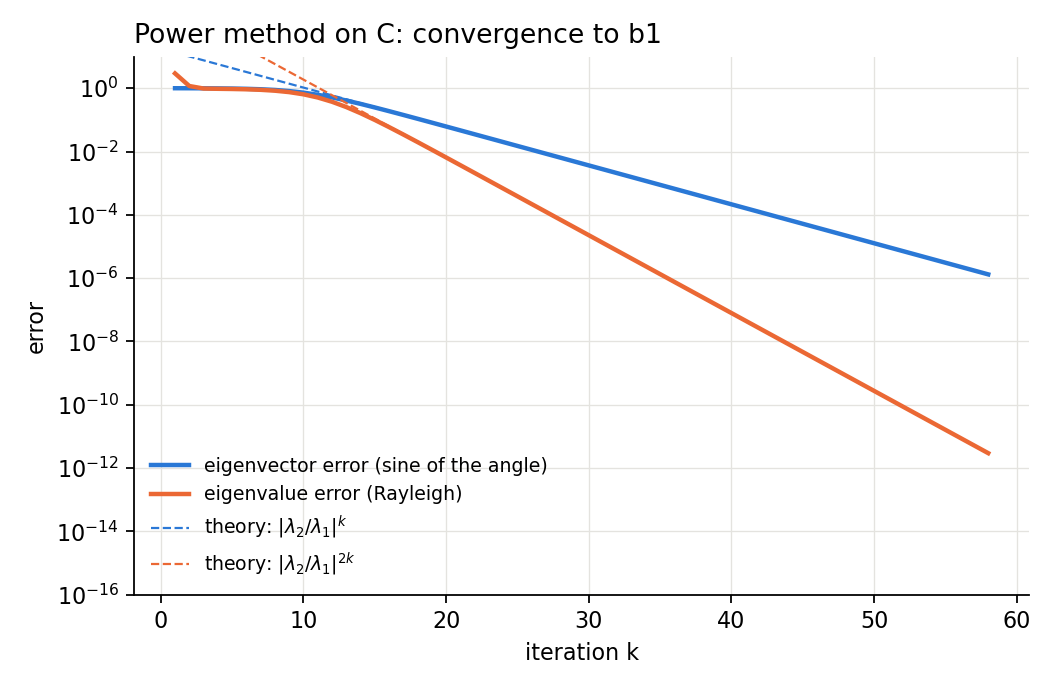
\includegraphics[width=0.72\textwidth]{fig_power_convergence.png}
\caption{Error of the power method for $\bb_1$: the curves are parallel to the theoretical lines
$|\lambda_2/\lambda_1|^k$ (eigenvector) and $|\lambda_2/\lambda_1|^{2k}$ (Rayleigh).}
\label{fig:pow}
\end{figure}

%=====================================================================
\section{Speeding up the method: shift and inverse iteration}
\paragraph{Shift.} $C-\sigma I$ has the same eigenvectors and eigenvalues $\lambda_i-\sigma$.
For $\bb_1$ the convergence ratio becomes $\max_{i\ge2}|\lambda_i-\sigma|/|\lambda_1-\sigma|$,
minimised by $\sigma^*=(\lambda_2+\lambda_D)/2$. With our data $\sigma^*=1.504$: the ratio drops
from $0.753$ to $0.601$ and the iterations from 47 to 29.

\paragraph{Shifted inverse power method.} $(C-\sigma I)^{-1}$ has eigenvalues $1/(\lambda_i-\sigma)$: the
eigenvalue closest to $\sigma$ dominates, with ratio
$|\lambda_j-\sigma|/|\lambda_{\text{next closest}}-\sigma|$. The inverse is never computed: at each step one solves
$(C-\sigma I)\mathbf w=\mathbf v$. The $LU$ factorisation (with pivoting) is computed \textbf{once},
and each iteration costs two triangular substitutions, $O(D^2)$ instead of $O(D^3)$.
\begin{center}
\begin{tabular}{ccccc}
\toprule
target & $\sigma$ & ratio & iterations & error on $\lambda$\\
\midrule
$\lambda_1$ & 3.8 & 0.175 & 9 & $2\cdot10^{-14}$\\
$\lambda_2$ & 3.0 & 0.029 & 5 & $9\cdot10^{-16}$\\
$\lambda_3$ & 1.0 & 0.171 & 8 & $1\cdot10^{-14}$\\
$\lambda_{10}$ & 0 & 0.476 & 20 & $3\cdot10^{-15}$\\
\bottomrule
\end{tabular}
\end{center}
With $\sigma=0$ one obtains the smallest eigenvalue (``pure'' inverse iteration).
By choosing $\sigma$, \emph{any} eigenvalue can be computed, without deflation.

\paragraph{What it is used for in the project: conditioning.}
With a $10\times10$ matrix speed is not an issue. The concrete use is another one:
the power method and inverse iteration with $\sigma=0$ give the extreme eigenvalues, and for a
symmetric positive definite matrix
\[
K_2(C)=\frac{\lambda_{\max}}{\lambda_{\min}}=\frac{3.945}{0.0364}=108.4,
\qquad
K_2(X)=\frac{\sigma_{\max}}{\sigma_{\min}}=10.41,\qquad K_2(X)^2=108.4 .
\]
This is the numerical check of $K_2(X^TX)=K_2(X)^2$ and it quantifies why the SVD of $X$ is preferred.
Moreover $\lambda_{\min}\approx 0$ says that along $\bb_{10}$ the players hardly vary: there is an almost
constant combination of statistics, i.e.\ some statistics are nearly redundant.

%=====================================================================
\section{Reliability of the axes}\label{sec:rel}
The data are perturbed with Gaussian noise equal to $10\%$ of the standard deviation (300 trials) and
the angle between each original eigenvector and the perturbed one is measured.
\begin{center}
\begin{tabular}{ccccc}
\toprule
axis & $\lambda_j$ & gap to neighbour & median rotation & 90\% rotation\\
\midrule
$\bb_1$ & 3.945 & 0.973 & $2.5^\circ$ & $5.1^\circ$\\
$\bb_2$ & 2.972 & 0.973 & $2.9^\circ$ & $5.3^\circ$\\
$\bb_3$ & 1.047 & 0.318 & $5.3^\circ$ & $9.2^\circ$\\
$\bb_4$ & 0.728 & 0.178 & $8.3^\circ$ & $13.6^\circ$\\
\bottomrule
\end{tabular}
\end{center}
The smaller the gap between an eigenvalue and its neighbours, the more \textbf{ill-conditioned} the eigenvector:
a small perturbation of the data makes it rotate a lot. In the limit $\lambda_j=\lambda_{j+1}$ the eigenvector is
not even defined (every direction in the plane is an eigenvector). It is the same gap that governs the
speed of the power method: \emph{slow convergence and instability have the same cause}.
This is why only $\bb_1$ and $\bb_2$ are interpreted.
\begin{figure}[h]
\centering
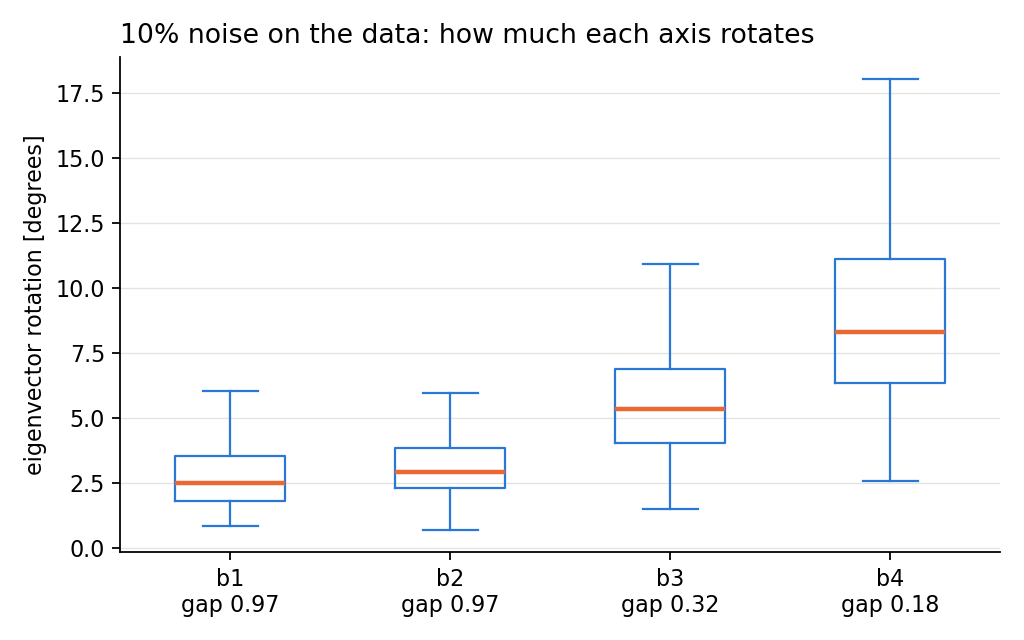
\includegraphics[width=0.55\textwidth]{fig_sensitivity.png}
\caption{Rotation of the eigenvectors with 10\% noise on the data: it grows as the gap shrinks.}
\end{figure}

%=====================================================================
\section{Rank $k$ and missing data}\label{sec:rank}
\paragraph{Eckart--Young.} Among rank-$k$ matrices, the closest to $X$ is
$X_k=U_k\Sigma_kV_k^T$, with
\[
\|X-X_k\|_2=\sigma_{k+1},\qquad \|X-X_k\|_F=\Big(\sum_{i>k}\sigma_i^2\Big)^{1/2}.
\]
Checked numerically for every $k$. Since $\sum_i\sigma_i^2=\|X\|_F^2$, we have
$\big(\|X-X_k\|_F/\|X\|_F\big)^2=1-\text{explained variance}$: with $k=3$ the relative error is
$45\%=\sqrt{1-0.796}$.

\paragraph{Imputation (the ``messy'' data).} Two players have 4 missing statistics. Instead of
replacing them with the mean, the low-rank structure is used: the statistics are correlated, so the
observed ones carry information about the missing ones. Fixed-point iteration: start with the holes equal
to the mean; at each step compute the rank-$k$ approximation and replace \emph{only} the missing values
with the reconstructed ones; stop when the imputed values no longer change.
Error on the missing values (RMSE, in standard deviations):
\begin{center}
\begin{tabular}{lccccc}
\toprule
method & mean & $k=1$ & $k=2$ & $k=3$ & $k=4$\\
\midrule
RMSE & 1.19 & 0.95 & \textbf{0.75} & 0.96 & 3.16 (does not converge)\\
\bottomrule
\end{tabular}
\end{center}
With small $k$ the imputation improves on the mean by $37\%$. With $k$ too large the model has enough
freedom to fit the observed data without constraining the missing ones: the fixed point becomes extremely slow or
does not converge, and the error blows up. Convergence, when it occurs, is linear (factor $0.915$ for $k=3$).
\begin{figure}[h]
\centering
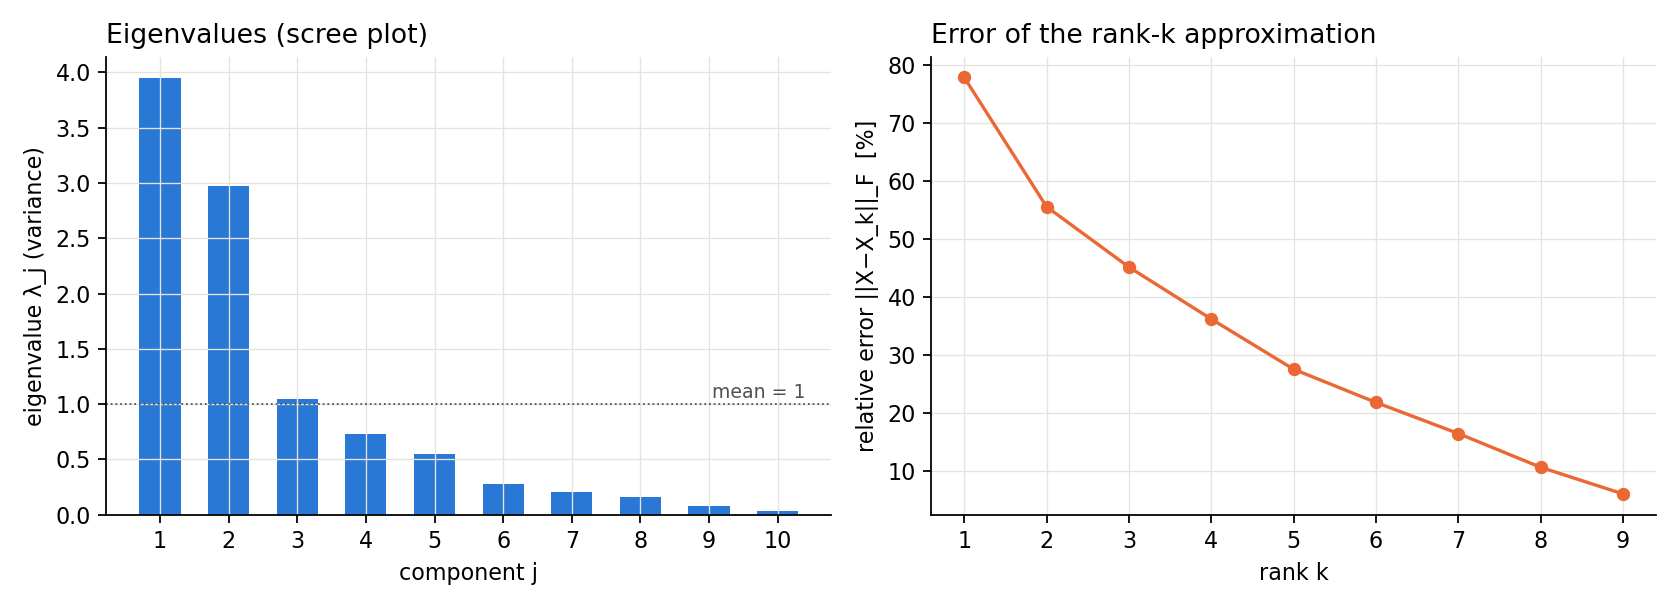
\includegraphics[width=0.9\textwidth]{fig_eckart_young.png}\\[4pt]
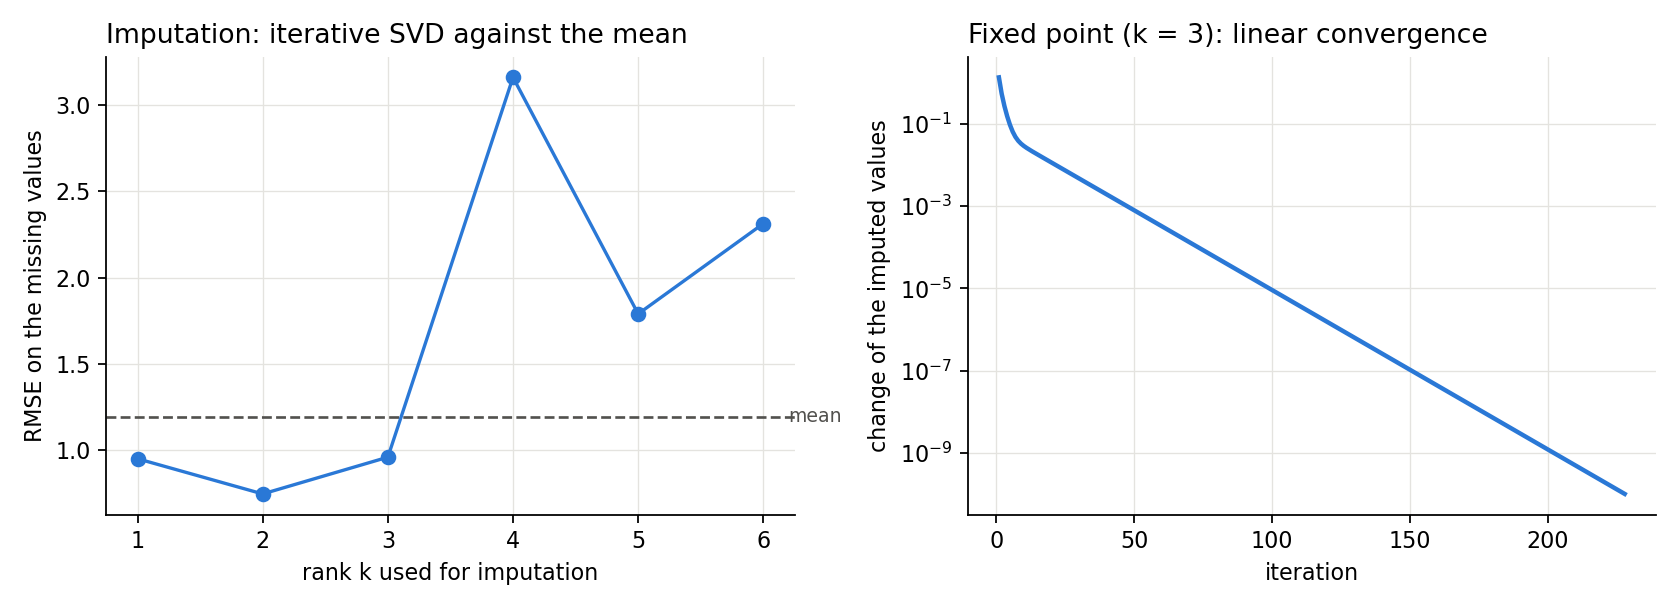
\includegraphics[width=0.9\textwidth]{fig_imputation.png}
\caption{Top: eigenvalues and rank-$k$ error. Bottom: imputation with iterative SVD and convergence of the fixed point.}
\end{figure}

%=====================================================================
\section{Interpreting the axes}
The name of an axis is read from its largest weights (loadings), positive and negative.
\begin{itemize}
\item $\bb_1$ \textbf{contact $\leftrightarrow$ wide game}: positive weights on rucks, tackles, lineouts;
negative on metres gained, defenders beaten, kicks. Props and locks on one side, wings and fullback on the other.
\item $\bb_2$ \textbf{ball carrier $\leftrightarrow$ low carrier}: positive weights on carries, offloads,
defenders beaten. On the opposite side there are both the playmakers and the props: the initial interpretation
``playmaker versus carrier'' was corrected by the data.
\end{itemize}
\begin{center}
\begin{tabular}{lrr@{\qquad}lrr}
\toprule
statistic & $\bb_1$ & $\bb_2$ & statistic & $\bb_1$ & $\bb_2$\\
\midrule
attacking rucks & $+0.48$ & $-0.04$ & carries & $+0.05$ & $+0.49$\\
tackles made & $+0.41$ & $+0.13$ & offloads & $-0.11$ & $+0.46$\\
dominant tackles & $+0.34$ & $+0.22$ & defenders beaten & $-0.33$ & $+0.38$\\
lineout jumps & $+0.32$ & $+0.02$ & metres gained & $-0.37$ & $+0.34$\\
passes & $-0.24$ & $-0.35$ & kicks in play & $-0.27$ & $-0.29$\\
\bottomrule
\end{tabular}
\end{center}
\begin{rem}
The axes describe \textbf{styles}, not levels: a low score on $\bb_1$ for a wing does not indicate a weakness.
To talk about room for improvement, players of the same role must be compared (Section~\ref{sec:dir}).
Moreover the third component is less reliable: $\lambda_3=1.05$ and $\lambda_4=0.73$ are close, and a small
gap between eigenvalues makes the eigenvector sensitive to noise in the data.
\end{rem}

%=====================================================================
\section{Balanced training groups}
Let $\z_n\in\R^{K}$ be the scores ($K=3$), with zero team mean. The players are split into
$G=5$ groups of 5; $\bar\z_g$ is the mean of group $g$ and $n_g$ the number of players.

\begin{prop}[Variance decomposition]
\[
\underbrace{\sum_n\|\z_n\|^2}_{SS_{\text{tot}}}
=\underbrace{\sum_g n_g\|\bar\z_g\|^2}_{SS_{\text{between}}}
+\underbrace{\sum_g\sum_{n\in g}\|\z_n-\bar\z_g\|^2}_{SS_{\text{within}}} .
\]
\end{prop}
\begin{proof}
For each group write $\z_n=(\z_n-\bar\z_g)+\bar\z_g$ and expand the square:
\[
\sum_{n\in g}\|\z_n\|^2=\sum_{n\in g}\|\z_n-\bar\z_g\|^2+n_g\|\bar\z_g\|^2
+2\,\bar\z_g^T\sum_{n\in g}(\z_n-\bar\z_g).
\]
The last sum is zero by definition of the mean. Summing over the groups gives the claim.
\end{proof}

\paragraph{Objective.}
$SS_{\text{tot}}$ is fixed by the data, hence
\[
\min SS_{\text{between}}\iff\max SS_{\text{within}} :
\]
groups with the same mean as the team are, necessarily, internally varied groups,
in which players strong and weak on every axis are mixed.
The axes must not be reweighted: the score along $\bb_j$ already has variance $\lambda_j$.

\paragraph{Swap algorithm.}
Start from a random split; try every swap of two players from different groups and
apply the one that decreases $SS_{\text{between}}$ the most; stop when no swap improves.
The algorithm finds a \textbf{local minimum}: it only accepts improving swaps and cannot get past
a configuration where it would first have to get worse. The possible splits are about
$25!/((5!)^5\,5!)\approx 5\cdot 10^{12}$, too many to explore; 30 random starts are used and the best is kept.

\paragraph{Results.}
$SS_{\text{tot}}=191.13$, $SS_{\text{between}}=0.30$ ($0.16\%$), $SS_{\text{within}}=190.83$; the sum satisfies
the identity to $10^{-14}$. Over 5000 random splits $SS_{\text{between}}$ has mean $31.7$ and minimum $4.2$
(Figure~\ref{fig:groups}). $SS_{\text{between}}$ does not reach 0 because every group would need a mean of
exactly zero on all three axes with exactly 5 players: in general this is not possible.

\begin{center}
\begin{tabular}{cl}
\toprule
group & players\\
\midrule
1 & Lock 3, Back row 1, Back row 5, Scrum-half 2, Wing 1\\
2 & Prop 3, Lock 1, Back row 2, Fly-half 2, Wing 2\\
3 & Prop 4, Hooker 2, Back row 3, Fly-half 1, Centre 2\\
4 & Hooker 1, Lock 2, Scrum-half 1, Centre 1, Wing 3\\
5 & Prop 1, Prop 2, Back row 4, Centre 3, Fullback 1\\
\bottomrule
\end{tabular}
\end{center}
Every group contains both forwards and backs, and in every group 2 or 3 players sit on each side of
$\bb_1$ and of $\bb_2$.

\begin{figure}[h]
\centering
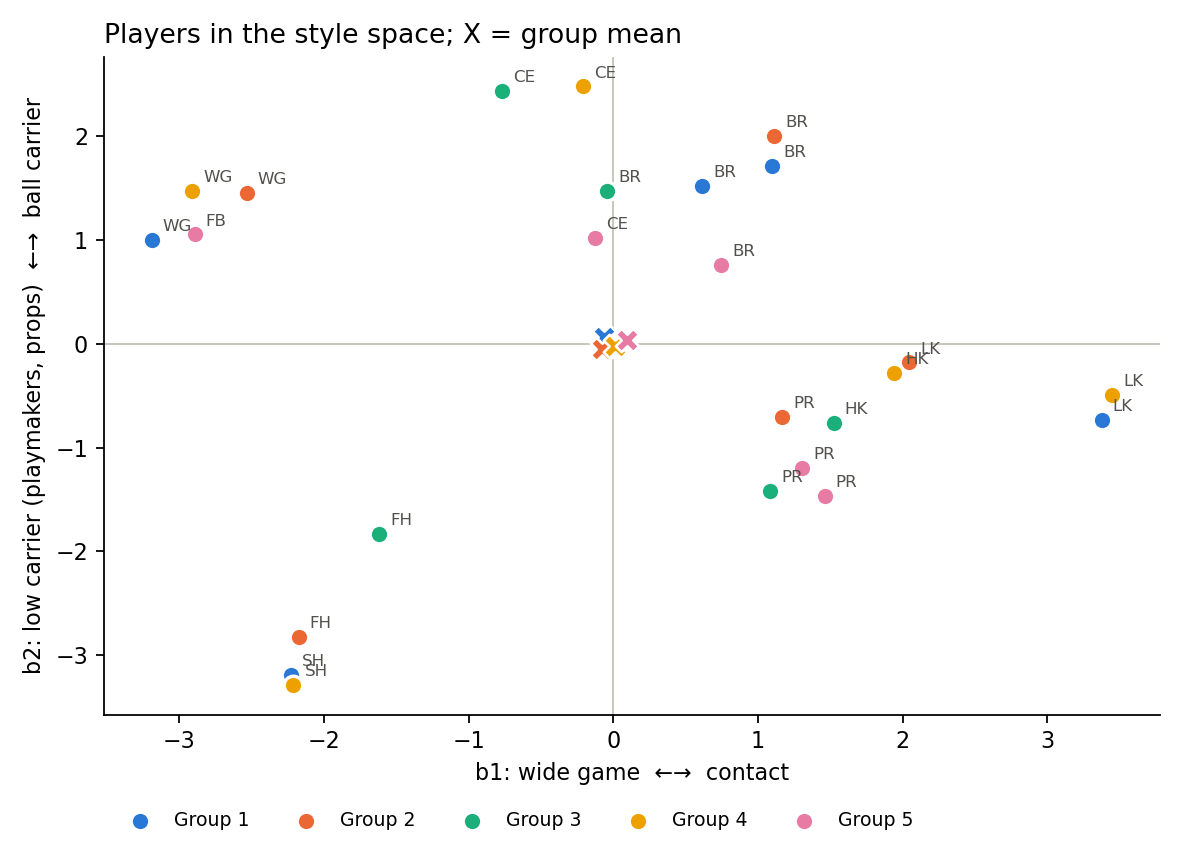
\includegraphics[width=0.49\textwidth]{fig_groups.png}\hfill
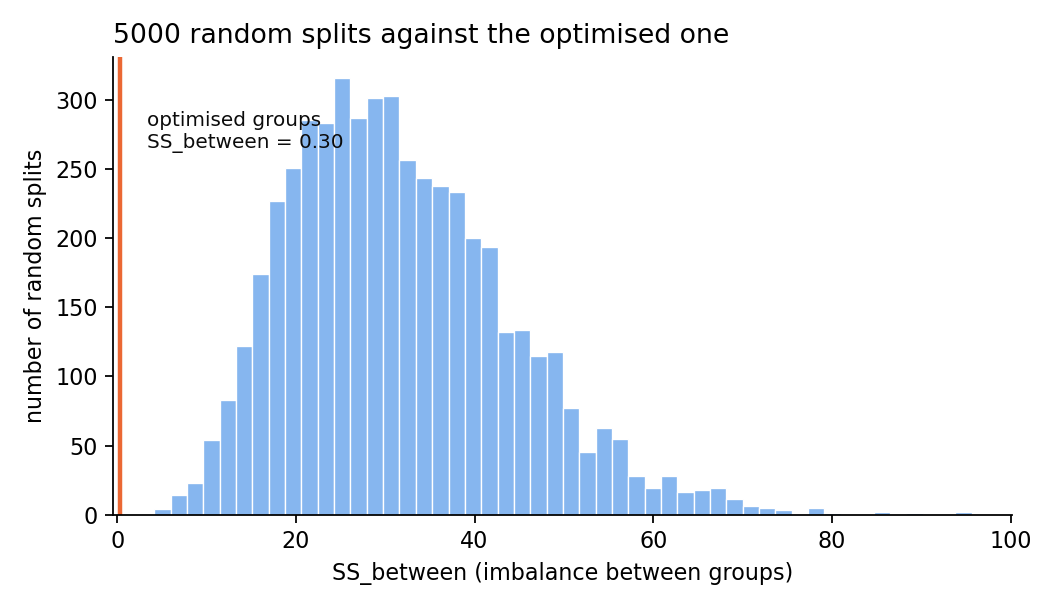
\includegraphics[width=0.49\textwidth]{fig_random_comparison.png}
\caption{Left: players in the $(\bb_1,\bb_2)$ plane coloured by group; the X marks are the group means,
all close to the origin. Right: $SS_{\text{between}}$ of 5000 random splits against the optimised split.}
\label{fig:groups}
\end{figure}

%=====================================================================
\section{Work directions}\label{sec:dir}
The groups answer the question \emph{who trains with whom}; this section answers \emph{what each
player should work on}. Since the axes describe styles and not levels, a raw score cannot be read
as ``good'' or ``bad'': a wing with a very negative $\bb_1$ score is doing exactly what a wing should do.
The reference for each player is therefore the \textbf{mean of their own role}. The procedure has three steps.

\subsection{Step 1: which axes characterise a role}
For each role $r$ we compute the mean score $\bar z_{r,j}$ on axis $j$ and measure it in units of the
standard deviation of the axis, $\sqrt{\lambda_j}$ (the score along $\bb_j$ has variance $\lambda_j$, so this
makes $\bb_1$ and $\bb_2$ comparable). An axis is used for role $r$ only if the role clearly sits on one
side of it, $|\bar z_{r,j}|\ge 0.5\sqrt{\lambda_j}$; its \emph{typical direction} is
$s=\operatorname{sign}(\bar z_{r,j})$.
\begin{center}
\begin{tabular}{lcrrl}
\toprule
role & players & $\bar z_{r,1}/\sqrt{\lambda_1}$ & $\bar z_{r,2}/\sqrt{\lambda_2}$ & axes used\\
\midrule
Prop & 4 & $+0.63$ & $-0.69$ & $\bb_1$ (contact), $\bb_2$ (low carrier)\\
Hooker & 2 & $+0.87$ & $-0.30$ & $\bb_1$\\
Lock & 3 & $+1.49$ & $-0.27$ & $\bb_1$\\
Back row & 5 & $+0.36$ & $+0.87$ & $\bb_2$ (carrier)\\
Scrum-half & 2 & $-1.12$ & $-1.88$ & $\bb_1$ (wide), $\bb_2$ (low carrier)\\
Fly-half & 2 & $-0.96$ & $-1.35$ & $\bb_1$, $\bb_2$\\
Centre & 3 & $-0.19$ & $+1.15$ & $\bb_2$\\
Wing & 3 & $-1.45$ & $+0.76$ & $\bb_1$, $\bb_2$\\
Fullback & 1 & $-1.46$ & $+0.61$ & $\bb_1$, $\bb_2$\\
\bottomrule
\end{tabular}
\end{center}
The table is itself a result: back-rowers and centres are not characterised by $\bb_1$ (they are the
``hybrid'' roles, halfway between contact and wide game) but they are the clearest ball carriers;
locks are the most extreme contact players; the halves are the least likely to carry.

\subsection{Step 2: the deficit}
For player $n$ of role $r$ and each axis $j$ used by the role,
\[
d_j=s\,\frac{z_{n,j}-\bar z_{r,j}}{\sqrt{\lambda_j}} .
\]
$d_j$ is measured in standard deviations of the axis. It is \textbf{positive} when the player is even more
pronounced than their role in the role's typical direction, \textbf{negative} when they are less so.
The axis with the most negative deficit is selected, and it is flagged only if $d_j<-0.25$.
The sign $s$ matters: for props the typical direction of $\bb_2$ is \emph{negative} (props carry little),
so a negative deficit for a prop means a prop who carries \emph{more} than the other props and does less of
the core work of the role. The direction of work is therefore ``towards the core of the role'', which is
not always ``more of everything''.

\subsection{Step 3: statistics to train and mentor}
The statistics to train are chosen among the six with the largest weight in direction $s$ of $\bb_j$,
keeping only those that (i) the role really uses (role mean above the team mean, so a prop is never told to
kick more) and (ii) in which the player is below the mean of their role; at most three are kept.
The mentor is the teammate \emph{in the same training group} who is strongest on those statistics.

This is where the two halves of the project meet. Minimising $SS_{\text{between}}$ forces every group to
contain players on both sides of each axis; therefore a player who is weak in a direction almost always
finds, in their own group, someone who is strong in that direction. Balanced groups are not only fair:
they are what makes in-group mentoring possible.

\subsection{Results}
\begin{center}
\begin{tabular}{llcll}
\toprule
player & group & axis ($d_j$) & to train & mentor\\
\midrule
Prop 3 & 2 & $\bb_2$ ($-0.28$) & attacking rucks & Lock 1\\
Lock 1 & 2 & $\bb_1$ ($-0.46$) & attacking rucks, tackles made, dominant tackles & Back row 2\\
Back row 4 & 5 & $\bb_2$ ($-0.43$) & carries, offloads, metres gained & Fullback 1\\
Fly-half 1 & 3 & $\bb_2$ ($-0.29$) & passes, kicks in play & Centre 2\\
Centre 3 & 5 & $\bb_2$ ($-0.56$) & carries, offloads, defenders beaten & Fullback 1\\
\bottomrule
\end{tabular}
\end{center}
\begin{itemize}
\item \textbf{Lock 1} is the clearest case on $\bb_1$: almost half a standard deviation less ``contact'' than the
other locks. Work on breakdown and defensive workload, with Back row 2, the player of group 2 who is strongest on those statistics.
\item \textbf{Back row 4} and \textbf{Centre 3} are the two hybrids who carry least compared with their role:
work on carrying, offloading and beating defenders. Both find their mentor in Fullback 1, in group 5.
\item \textbf{Prop 3} and \textbf{Fly-half 1} are flagged on $\bb_2$ with the ``reversed'' sign described above:
they drift away from the low-carrier profile of their role, so the indication is to reinforce the core
tasks (rucks for the prop; passing and kicking for the fly-half).
\end{itemize}
The other 20 players have no deficit below $-0.25$. The full list of deficits also shows the
\textbf{strengths}, which identify natural mentors: Back row 2 ($d_2=+0.30$), Centre 1 ($+0.29$),
Fly-half 2 ($+0.29$), Centre 2 ($+0.27$), Lock 2 ($d_1=+0.25$).

\subsection{How to read these results: caveats}
\begin{itemize}
\item \textbf{Small roles.} The role mean is estimated on very few players. The only fullback is the mean of
their role, so their deficit is identically $0$: the method is blind on that player. With two players the deficits are
exactly opposite ($\pm0.29$ for the fly-halves): if two players of a role differ enough, one of them is always flagged,
even if both are good.
\item \textbf{Thresholds.} The values $0.5\sqrt{\lambda_j}$ (role characterised by an axis) and $-0.25$ (deficit worth
flagging) are modelling choices, not consequences of the theory. Prop 3 ($-0.28$) and Fly-half 1 ($-0.29$) are close
to the threshold; Lock 1, Back row 4 and Centre 3 are robust indications.
\item \textbf{Archetype assumption.} The direction of work pushes each player towards the typical profile of their role.
A coach might want the opposite (for instance a prop who carries more); in that case the role mean should be replaced
by a target profile chosen by the coach, and the same formula applies.
\item \textbf{Only two axes.} $\bb_3$ is not used because its direction is unstable (Section~\ref{sec:rel}).
\item \textbf{Mentor load.} The rule does not limit how many players share a mentor: Fullback 1 mentors two
teammates in group 5.
\end{itemize}

\subsection{Next steps for the work directions}
\begin{enumerate}
\item \textbf{Monitoring over time.} Freeze the transformation (means $\mu_j$, standard deviations $\sigma_j$ and
axes $B$ of the reference season) and project the new data of each training block onto it:
$\z_n^{(t)}=B^T\big((\x_n^{(t)}-\boldsymbol\mu)/\boldsymbol\sigma\big)$. The deficit $d_j^{(t)}$ then becomes
a progress indicator that is comparable across time. Recomputing the PCA every time would rotate the axes
(by a few degrees, Section~\ref{sec:rel}) and mix real improvements with changes of reference.
\item \textbf{Uncertainty on the deficit.} The same perturbation experiment used for the axes can be applied to the
deficits: flag a player only if $d_j<-0.25$ in, say, 90\% of the perturbed datasets. This would separate robust
indications from borderline ones automatically.
\item \textbf{More reliable role means.} For small roles, shrink the role mean towards the mean of the unit
(forwards/backs), or estimate the role means on league data while keeping the groups inside the squad.
\item \textbf{Mentor-aware groups.} Add a term to the swap objective that penalises a group in which a flagged player
has no teammate stronger on their statistics, or in which one mentor has more than one mentee. The swap algorithm
does not change: only the function evaluated at each swap does.
\item \textbf{Match-level data.} Season averages hide variability between matches; with per-match data each player
becomes a cloud of points, and the distance from the role mean can be measured against the player's own variability.
\end{enumerate}

%=====================================================================
\section{Limitations}
\begin{itemize}
\item Synthetic data, $N=25$: the components beyond the second are not very reliable (Section~\ref{sec:rel}).
\item The swap algorithm is a heuristic: there is no guarantee of a global optimum.
\item PCA describes styles, not levels: the work direction requires additional assumptions
(comparison with the role, Section~\ref{sec:dir}).
\item Developments: real data from a whole league (axes estimated on many players, groups inside one team);
for large $N$ the product $C\mathbf v=X^T(X\mathbf v)/(N-1)$ avoids forming $C$.
\end{itemize}

\begin{thebibliography}{9}
\bibitem{mml} M. P. Deisenroth, A. A. Faisal, C. S. Ong, \emph{Mathematics for Machine Learning}, Cambridge University Press, 2020. Ch. 6 (summary statistics, geometry of random variables) and ch. 10 (PCA).
\end{thebibliography}

\end{document}
